\let\negmedspace\undefined
\let\negthickspace\undefined
\documentclass[journal]{IEEEtran}
\usepackage[a5paper, margin=10mm, onecolumn]{geometry}
%\usepackage{lmodern} % Ensure lmodern is loaded for pdflatex
\usepackage{tfrupee} % Include tfrupee package

\setlength{\headheight}{1cm} % Set the height of the header box
\setlength{\headsep}{0mm}     % Set the distance between the header box and the top of the text

\usepackage{gvv-book}
\usepackage{gvv}
\usepackage{cite}
\usepackage{amsmath,amssymb,amsfonts,amsthm}
\usepackage{algorithmic}
\usepackage{graphicx}
\usepackage{textcomp}
\usepackage{xcolor}
\usepackage{txfonts}
\usepackage{listings}
\usepackage{enumitem}
\usepackage{mathtools}
\usepackage{gensymb}
\usepackage{comment}
\usepackage[breaklinks=true]{hyperref}
\usepackage{tkz-euclide} 
\usepackage{listings}
\usepackage{gvv}                                        
\def\inputGnumericTable{}                                 
\usepackage[latin1]{inputenc}                                
\usepackage{color}                                            
\usepackage{array}                                            
\usepackage{longtable}                                       
\usepackage{calc}                                             
\usepackage{multirow}                                         
\usepackage{hhline}                                           
\usepackage{ifthen}                                           
\usepackage{lscape}
\usepackage{circuitikz}
\tikzstyle{block} = [rectangle, draw, fill=blue!20, 
    text width=4em, text centered, rounded corners, minimum height=3em]
\tikzstyle{sum} = [draw, fill=blue!10, circle, minimum size=1cm, node distance=1.5cm]
\tikzstyle{input} = [coordinate]
\tikzstyle{output} = [coordinate]

\begin{document}


\bibliographystyle{IEEEtran}
\vspace{3cm}

\title{9.2.11}
\author{EE25BTECH11049 - Sai Krishna Bakki}
 \maketitle
% \newpage
% \bigskip
{\let\newpage\relax\maketitle}

\renewcommand{\thefigure}{\theenumi}
\renewcommand{\thetable}{\theenumi}
\setlength{\intextsep}{10pt} % Space between text and floats


\numberwithin{equation}{enumi}
\numberwithin{figure}{enumi}
\renewcommand{\thetable}{\theenumi}
\textbf{Question:}\\
Find the area of the region bounded by the curve $y^2 = 9x$ and the lines $x = 2$ and $x = 4$ and the x-axis in the first quadrant.\\

\solution\\
The general equation of a conic section is given by $\vec{x}^\top\vec{V}\vec{x} + 2\vec{u}^\top\vec{x} + f = 0$, where $\vec{x} = \myvec{x \\ y}$.
The parameters of the conic are
\begin{align}
\vec{V} = \myvec{0 & 0 \\ 0 & 1}, \quad \vec{u} = \myvec{-9/2 \\ 0}, \quad f = 0
\end{align}

For the line x - 2 = 0, the parameters are
\begin{align}
\vec{h}_1 = \myvec{2 \\ 0}, \quad \vec{m}_1 = \myvec{0 \\ 1}
\end{align}
The parameter $\kappa$ for the points of intersection is found using the formula:
\begin{align}
\kappa = \frac{1}{\vec{m}^\top \vec{V} \vec{m}}\brak{-\vec{m}^\top(\vec{V}\vec{h}+\vec{u}) \pm \sqrt{\sbrak{\vec{m}^\top(\vec{V}\vec{h}+\vec{u})}^2 - g(\vec{h})(\vec{m}^\top \vec{V} \vec{m})}}
\end{align}
where $g(\vec{h}) = \vec{h}^\top \vec{V} \vec{h} + 2\vec{u}^\top \vec{h} + f$.

% First, we compute the value of $g(\vec{h}_1)$:
% \begin{align*}
% g(\vec{h}_1) &= \myvec{2 & 0} \myvec{0 & 0 \\ 0 & 1} \myvec{2 \\ 0} + 2 \myvec{-9/2 & 0} \myvec{2 \\ 0} + 0 \\
% &= -18
% \end{align*}
% Next, we compute the other components needed for the $\kappa$ formula:
% \begin{align*}
% \vec{m}_1^\top \vec{V} \vec{m}_1 &= \myvec{0 & 1} \myvec{0 & 0 \\ 0 & 1} \myvec{0 \\ 1} = 1 \\
% \vec{m}_1^\top(\vec{V}\vec{h}_1+\vec{u}) &= \myvec{0 & 1} \brak{\myvec{0 & 0 \\ 0 & 1} \myvec{2 \\ 0} + \myvec{-9/2 \\ 0}} = \myvec{0 & 1}\myvec{-9/2 \\ 0} = 0
% \end{align*}
Substituting the values into the formula for $\kappa$:
\begin{align}
\kappa &= \brak{-0 \pm \sqrt{0^2 - (-18)(1)}} = 3\sqrt{2},-3\sqrt{2}
\end{align}
yielding the points of intersection
\begin{align}
\vec{a}_0 =  \myvec{2 \\ 3\sqrt{2}},\vec{a}_1 =  \myvec{2 \\ -3\sqrt{2}}
\end{align}

For the line x - 4 = 0, the parameters are:
\begin{align}
\vec{h}_2 = \myvec{4 \\ 0}, \quad \vec{m}_2 = \myvec{0 \\ 1}
\end{align}
% We compute $g(\vec{h}_2)$:
% \begin{align*}
% g(\vec{h}_2) &= \myvec{4 & 0} \myvec{0 & 0 \\ 0 & 1} \myvec{4 \\ 0} + 2 \myvec{-9/2 & 0} \myvec{4 \\ 0} + 0 = -36
% \end{align*}
% The remaining components are computed similarly: $\vec{m}_2^\top \vec{V} \vec{m}_2 = 1$ and $\vec{m}_2^\top(\vec{V}\vec{h}_2+\vec{u}) = 0$.
\begin{align}
\kappa &= \frac{1}{1}\brak{-0 \pm \sqrt{0^2 - (-36)(1)}} = 6,-6
\end{align}
yielding the points of intersection
\begin{align}
\vec{a}_2 = \myvec{4 \\ 6},\vec{a}_3 = \myvec{4 \\ -6}
\end{align}
Thus, the area of the parabola in between the lines x = 2 and
x = 4 is given by
\begin{align}
A &= \int_{0}^{4} 3\sqrt{x} \, dx -\int_{0}^{2} 3\sqrt{x}\,dx  \\
% &= 3 \int_{2}^{4} x^{1/2} \, dx \\
% &= 3 \sbrak{ \frac{x^{3/2}}{3/2} }_{2}^{4} \\
% &= 2 \sbrak{ x^{3/2} }_{2}^{4} \\
% &= 2 \brak{ 4^{3/2} - 2^{3/2} } \\
% &= 2 \brak{ (2^2)^{3/2} - 2\sqrt{2} } \\
% &= 2(8 - 2\sqrt{2}) \\
&= 16 - 4\sqrt{2}
\end{align}
Thus, the area of the specified region is 16 - 4$\sqrt{2}$ square units.
    \begin{figure}[H]
    \centering
    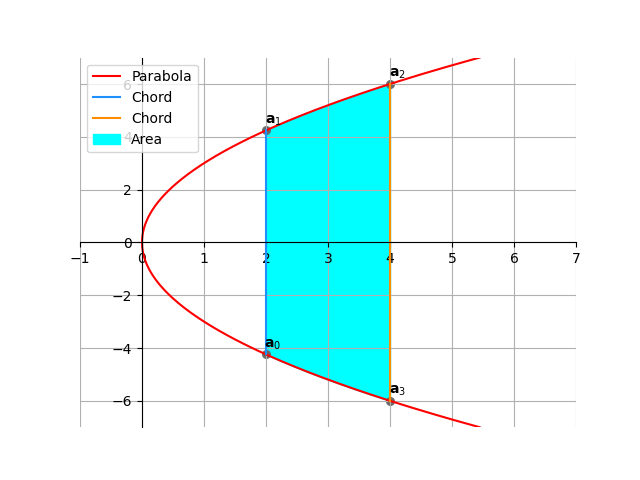
\includegraphics[width=0.7\columnwidth]{figs/Figure_1.png}
    \label{fig:placeholder}
    \caption{}
\end{figure}

\end{document}
